\documentclass{scrreprt}

\usepackage{aligned-overset}
\usepackage{amsmath}
\usepackage{amssymb}
\usepackage{bm}
\usepackage[shortlabels]{enumitem}
\usepackage{hyperref}
\usepackage[utf8]{inputenc}
\usepackage{mathtools}
\usepackage{physics}
\usepackage{tabularx}
\usepackage{titling}
\usepackage{fancyhdr}
\usepackage{xfrac}
\usepackage{pgfplots}

\pgfplotsset{compat = newest}
\usepgfplotslibrary{fillbetween}

\author{}
\date{SoSe 2021}
\title{Hausaufgabe 08 \\Analysis - Weiterführende Konzepte}

\setlength{\headheight}{26pt}
\pagestyle{fancy}
\fancyhf{}
\lhead{\thetitle}
\rhead{\theauthor}
\lfoot{\thedate}
\rfoot{Seite \thepage}

\begin{document}
\paragraph{Hausaufgabe 2} Gegeben sei die Funktion
$f \colon \mathbb{R}^2 \to \mathbb{R}$ mit
\begin{flalign*}
  f(x) &\coloneqq \begin{cases}
    \frac{x_1x_2}{\sqrt{x_1^2 + x_2^2}}, & \text{für } x = \qty(x_1, x_2) \ne (0, 0) \\
    0, & \text{für } x = (0, 0)
  \end{cases} &
\end{flalign*}
\begin{center}
  \resizebox{.8\textwidth}{!}{
    \begin{tikzpicture}[
        declare function={
          f(\x, \y) = \x^2 + \y^2 != 0 ? (\x*\y)/(sqrt(\x^2 + \y^2)) : 0;
        }
      ]
      \begin{axis}[
        xlabel = $x$,
        ylabel = $y$,
        view={20}{40},
      ]
        \addplot3[
          surf,
          domain=-1:1,
          samples=25,
          shader=faceted interp,
        ] {f(x, y)};
      \end{axis}
    \end{tikzpicture}
  }
\end{center}

\begin{enumerate}[a)]
\item Zeigen Sie, dass $f$ in $(0, 0)$ stetig ist.
  \subparagraph{Lösung:} Die Funktion $f$ heißt stetig im Punkt
  $x_0 = (0, 0) \in \mathbb{R}^2$, wenn
  \begin{flalign*}
    \forall \epsilon > 0 \:\exists\: \delta > 0 \forall y \in \mathbb{R}^2 \colon \norm{x_0 - y}_2 < \delta
    &\Rightarrow \abs{f(x_0) - f(y)} < \epsilon & \\
    \sqrt{y_1^2 + y_2^2} < \delta &\Rightarrow \abs{\frac{y_1y_2}{\sqrt{y_1^2 + y_2^2}}} < \epsilon \\
    \sqrt{y_1^2 + y_2^2} < \delta &\Rightarrow \frac{\abs{y_1y_2}}{\sqrt{y_1^2 + y_2^2}} < \epsilon \\
    \sqrt{y_1^2 + y_2^2} < \delta &\Rightarrow \sqrt{y_1^2 + y_2^2} \cdot \frac{\abs{y_1y_2}}{y_1^2 + y_2^2} < \epsilon \\
    \sqrt{y_1^2 + y_2^2} < \delta &\Rightarrow \sqrt{y_1^2 + y_2^2} \cdot \frac{1}{\abs{\frac{y_1}{y_2}} + \abs{\frac{y_2}{y_1}}}
    \leq \frac{\sqrt{y_1^2 + y_2^2}}{2} < \epsilon
  \end{flalign*}
  $\Rightarrow f$ ist im Punkt $(0, 0)$ stetig mit $\delta > 2\epsilon$.

\end{enumerate}

\end{document}